\documentclass[12pt]{beamer}

\hypersetup{colorlinks=true,linkcolor = blue}
\usetheme{Warsaw}

\usepackage[utf8]{inputenc}
\usepackage[russian,english]{babel}
\usepackage[T2A]{fontenc}

\usepackage{hyperref}
\usepackage[final]{listings}
\usepackage{breakurl}
\usepackage{cite}
\usepackage{perpage}

\def\Url\Breaks{\do\/\do-}

\lstset{
  frame=single,
  breaklines=true,
  basicstyle=\small,
  postbreak=\raisebox{0ex}{\ensuremath{\hookrightarrow\space}},
  numbers=left
}

\MakePerPage{footnote}

\title{Operating Systems}
\subtitle{Memory Allocation}
\author{Me}
\date{\today}

\begin{document}

  \begin{frame}
    \titlepage
  \end{frame}

  \begin{frame}
\frametitle{План}

\begin{enumerate}
  \item Расположение физической памяти.
  \item Понятие процесса и виртуальная память.
  \item Сегментация памяти как способ защиты.
  \item Paging и Page Fault.
  \item Аллокация непоследовательных страниц.
\end{enumerate}
\end{frame}

  \begin{frame}
\frametitle{Классы памяти}

\onslide<1->{По привелегиям доступа:
\begin{enumerate}
  \item привелигерованная (kernel space)
  \item не привелигерованная (user space)
\end{enumerate}}

\onslide<2->{По способу аллокации:
\begin{enumerate}
  \item статическая память (код, глобальные перменные - размер известен заранее)
  \item динамическая память (куча, free store и тд - размер не известен заранее)
\end{enumerate}}
\end{frame}

\begin{frame}
\frametitle{Карта памяти}

\begin{columns}[T]

  \begin{column}{.4\textwidth}
    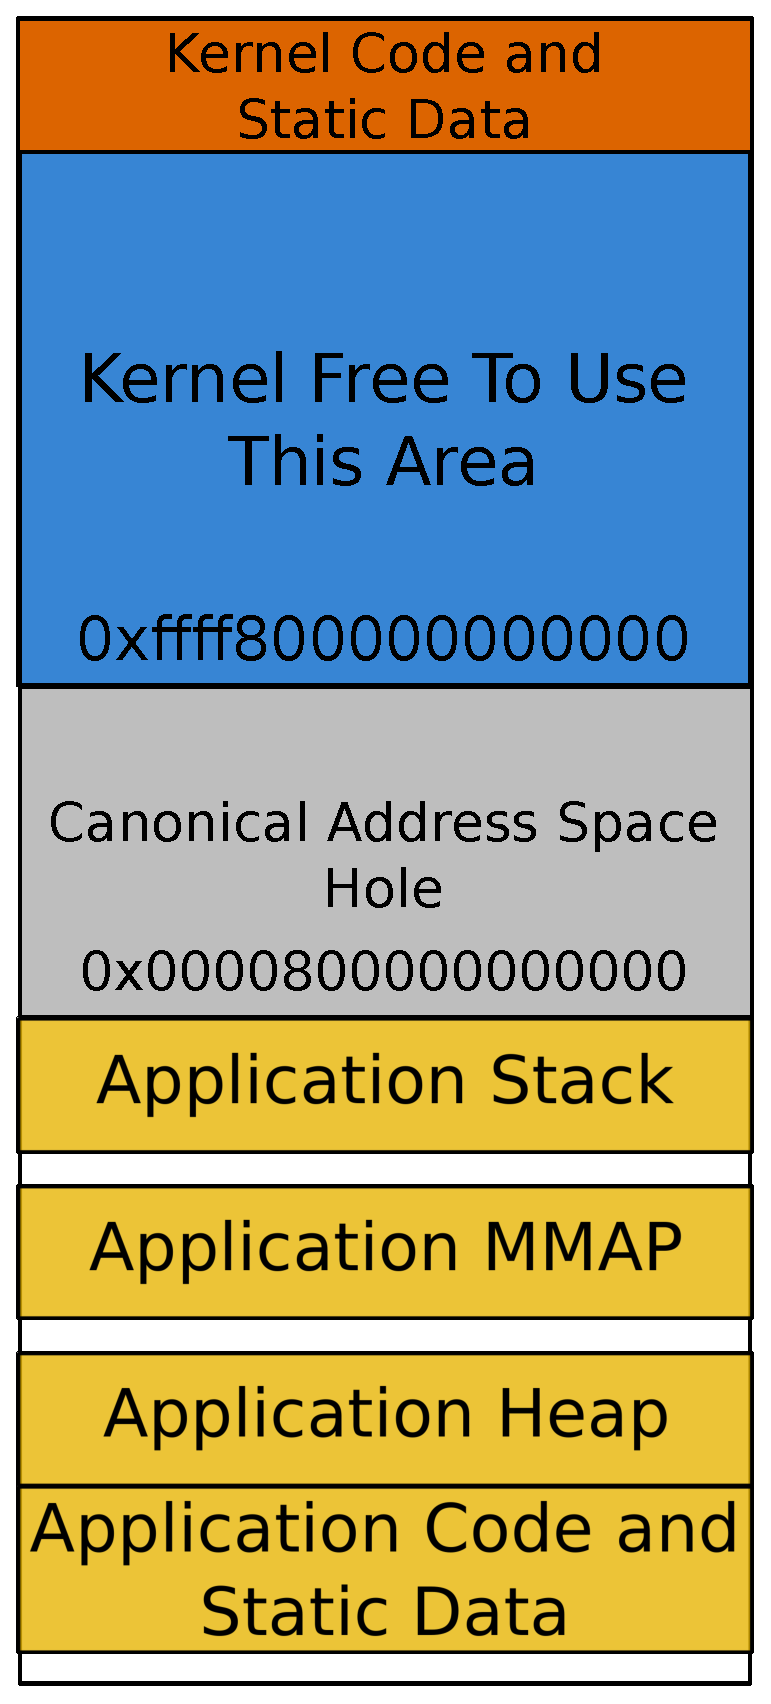
\includegraphics[width=.8\linewidth]{memmap}
  \end{column}

  \begin{column}{.6\textwidth}
    \begin{itemize}
      \item Kernel Code and Static Data - привелигерованная статическая память (System V ABI amd64, 3.5.1 Architectural Constraints, Kernel code model)
      \item Canonical Address Space Hole - недопустимые адреса памяти (Intel\textsuperscript{\textregistered} 64 and IA-32 Architectures Software Developer's Manual, 3.3.7.1 Canonical Addressing)
    \end{itemize}
  \end{column}
\end{columns}

\end{frame}

\begin{frame}
\frametitle{Карта памяти}

\begin{columns}[T]

  \begin{column}{.4\textwidth}
    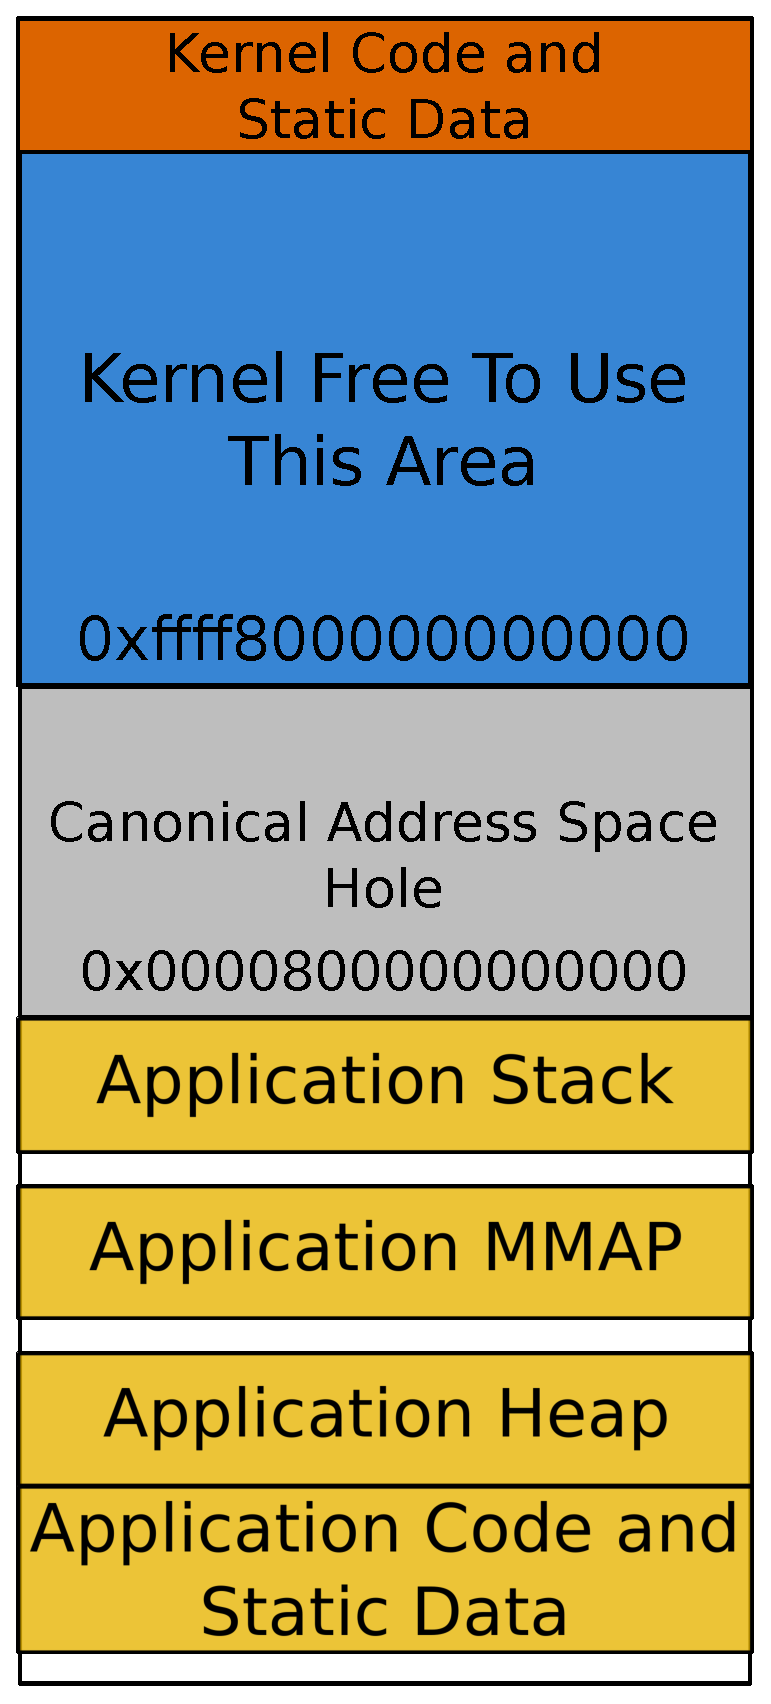
\includegraphics[width=.8\linewidth]{memmap}
  \end{column}

  \begin{column}{.6\textwidth}
    \begin{itemize}
      \item Application Stack - аллоцируется ОС при старте программы
      \item Application MMAP - разделяемые библиотеки, mmap/munmap
      \item Application Heap - malloc берет память отсюда, изменяется системным вызовом sbrk
      \item Application Code and Static Data - статическая не привелигерованная память
    \end{itemize}
  \end{column}
\end{columns}

\end{frame}


  \begin{frame}
\frametitle{Простые алгоритмы аллокации памяти}
\framesubtitle{Постановка задачи}

Чего мы хотим:
\begin{itemize}
  \item<2-> реализовать malloc и free
  \item<3-> чем быстрее тем лучше
  \item<4-> избежать фрагментации памяти, если получится
\end{itemize}
\end{frame}

\begin{frame}
\frametitle{Простые алгоритмы аллокации памяти}
\framesubtitle{Постановка задачи}

\onslide<1->{
Исходные данные - участок памяти:
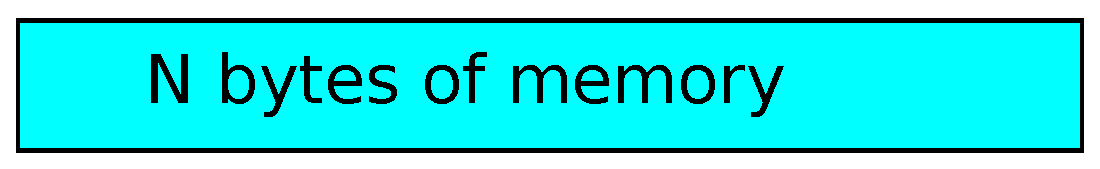
\includegraphics[width=0.9\linewidth]{alloc-basic0}}

\onslide<2->{и, для удобства, какая-то память константного размера:
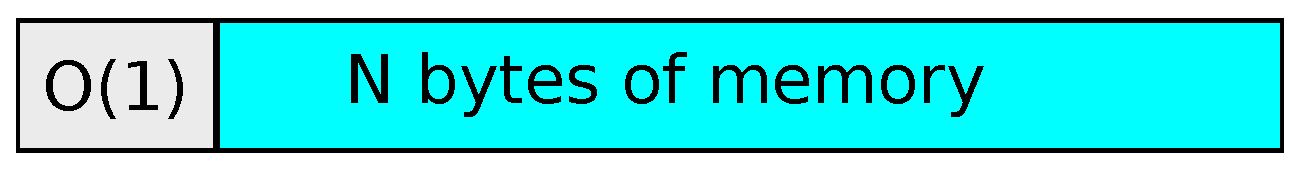
\includegraphics[width=0.9\linewidth]{alloc-basic1}}

\end{frame}

\begin{frame}
\frametitle{Простые алгоритмы аллокации памяти}
\framesubtitle{Аллокация}

Построим в памяти связный список свободных участков:

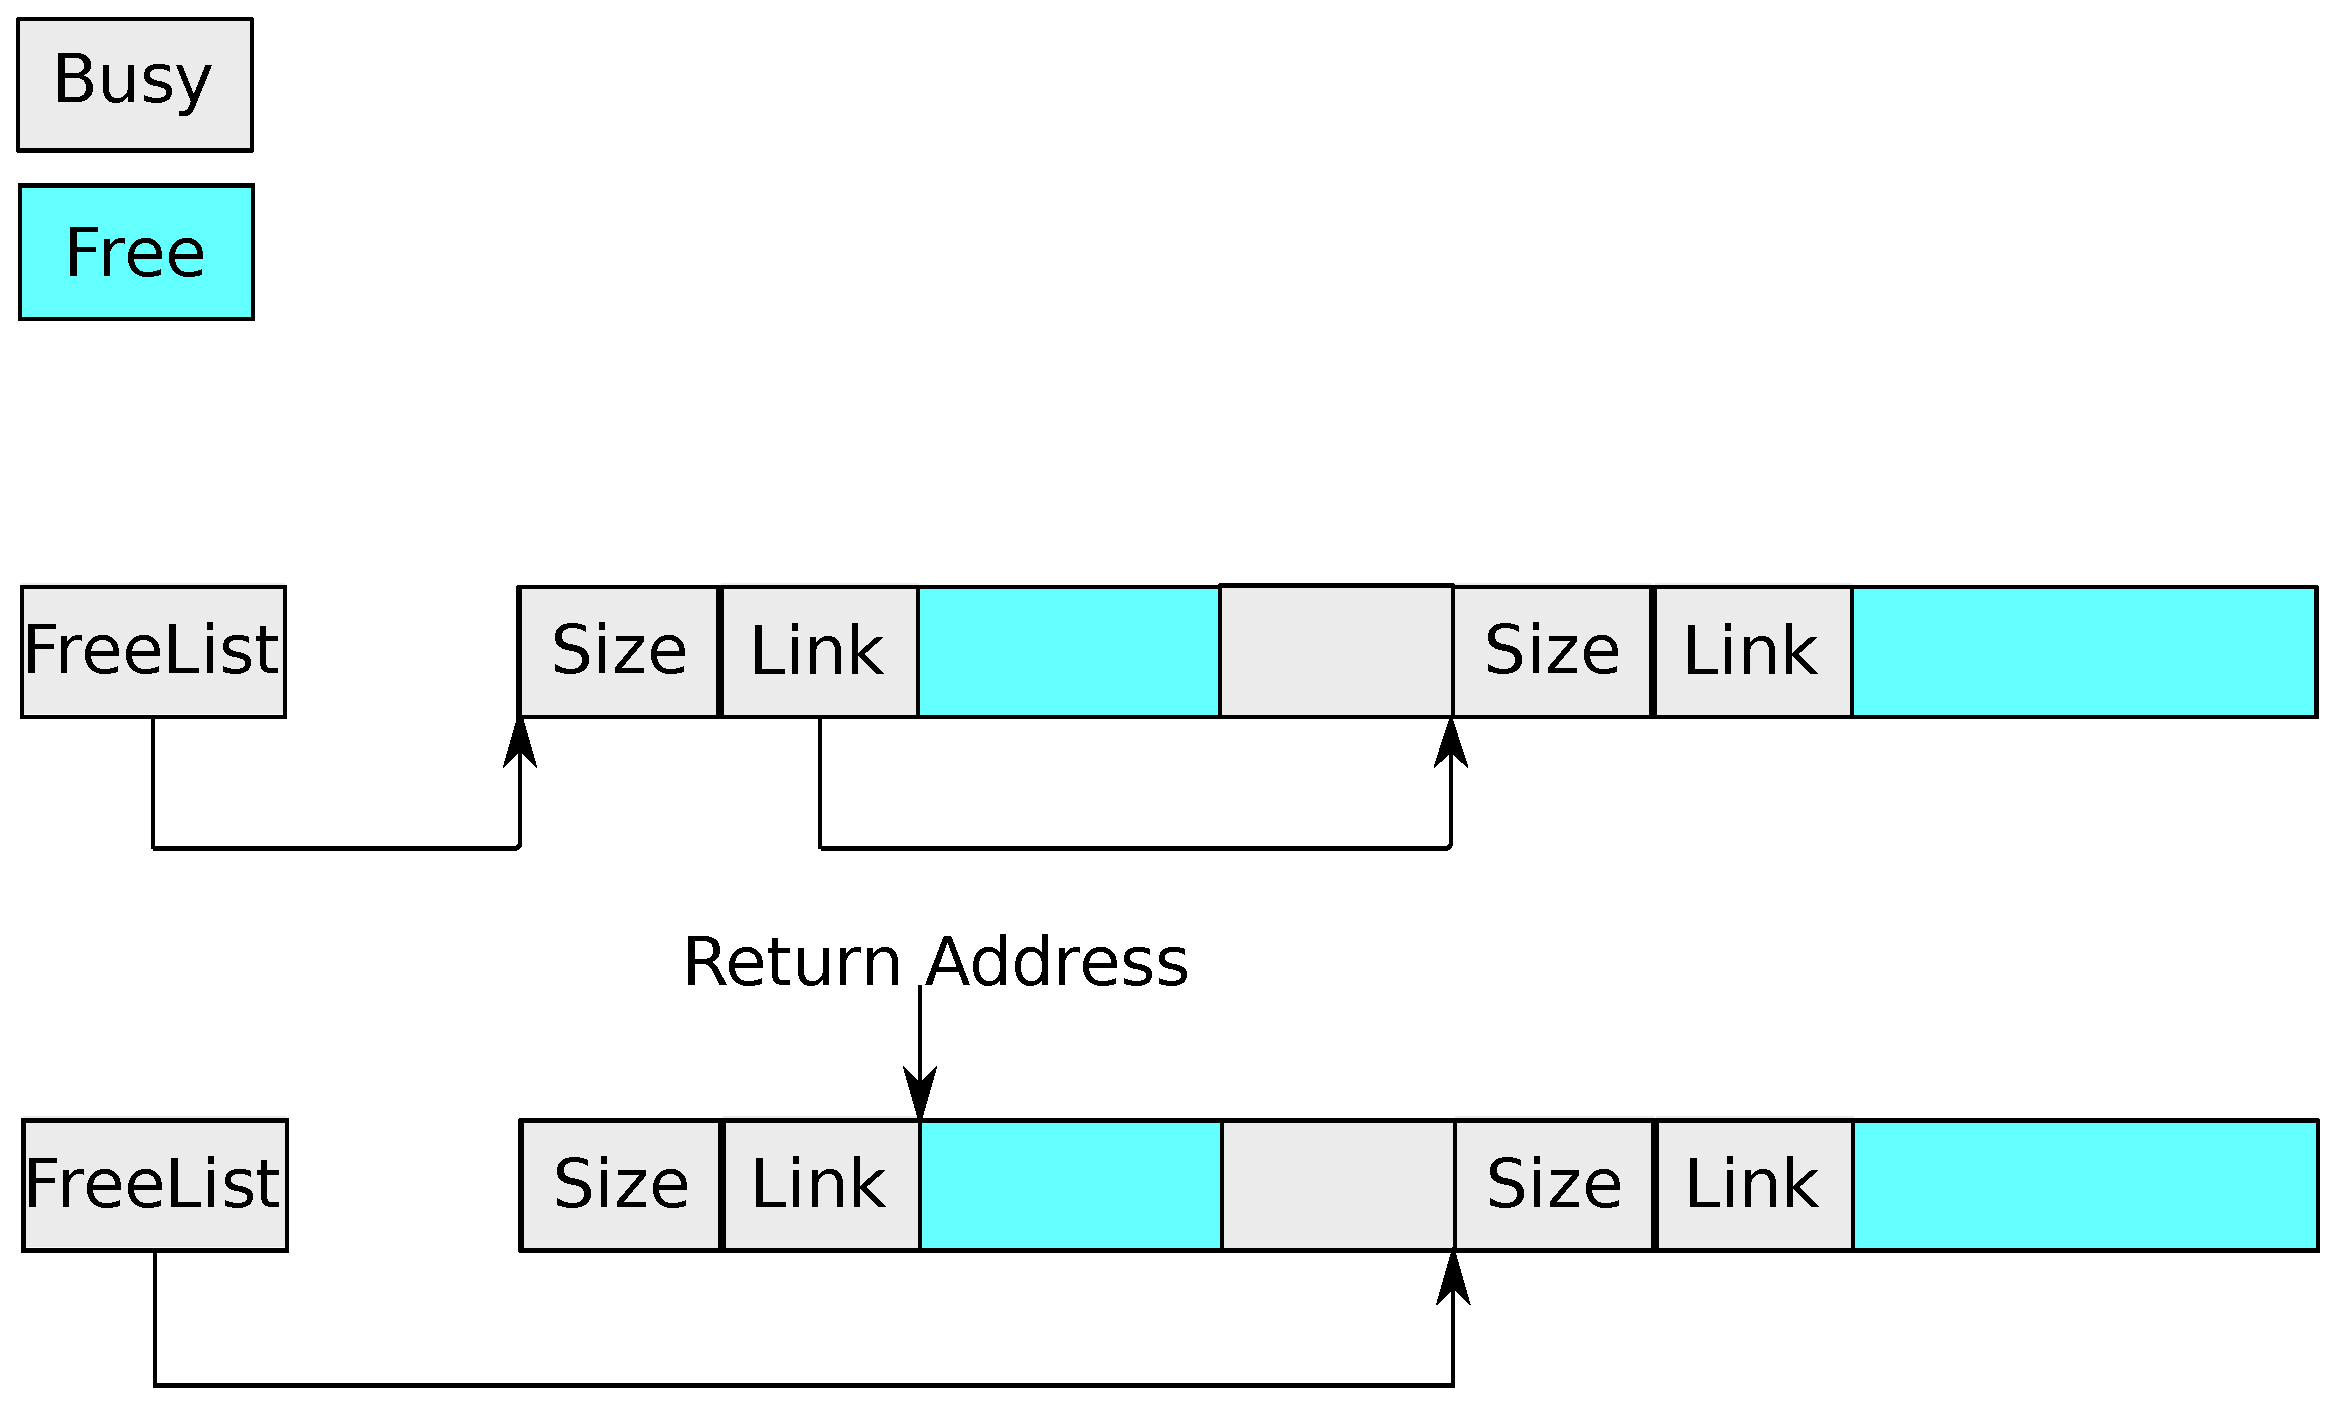
\includegraphics[width=.9\linewidth]{alloc-alloc0}
\end{frame}

\begin{frame}
\frametitle{Простые алгоритмы аллокации памяти}
\framesubtitle{Аллокация}

\onslide<1->{При аллокации проходим список свободных участков и выбираем подходящий.}

\onslide<2->{Как выбрать подходящий?}
\begin{itemize}
  \item<3-> Best Fit - проходим весь список, выбираем наименьший из подходящих
  \item<4-> First Fit - выбираем из списка первый подходящий
\end{itemize}

\onslide<5->{Какая стратегия лучше?}
\begin{enumerate}
  \item<6-> науке это не известно - разные приложения используют память по разному
  \item<7-> зачастую First Fit лучше - не нужно проходить весь список при прочих равных (неизвестных)
  \item<8-> простые алгоритмы редко используются на практике - есть лучшие подходы
\end{enumerate}
\end{frame}

\begin{frame}
\frametitle{Простые алгоритмы аллокации памяти}
\framesubtitle{Аллокация}

Почему бы пользователю не запоминать размер аллоцируемого блока? В простых случаях это будет работать хорошо:
\begin{itemize}
  \item часто размер известен в момент компиляции (sizeof(...))
  \item часто размер объекта вам нужен сам по себе - можно избежать дублирования
  \item пользователь сам определяет, где и как хранить размер
\end{itemize}
\end{frame}

\begin{frame}
\frametitle{Простые алгоритмы аллокации памяти}
\framesubtitle{Аллокация}

Однако в нашем случае это не будет работать - аллоцированный блок может быть больше запрошенного:

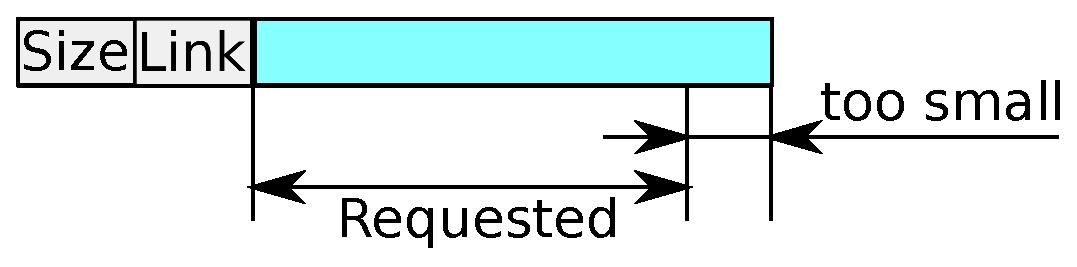
\includegraphics[width=.9\linewidth]{alloc-alloc1}
\end{frame}

\begin{frame}
\frametitle{Простые алгоритмы аллокации памяти}
\framesubtitle{Освобождение}

Функция освобождения принимает указатель как аргумент, нам так же нужен размер участка памяти:

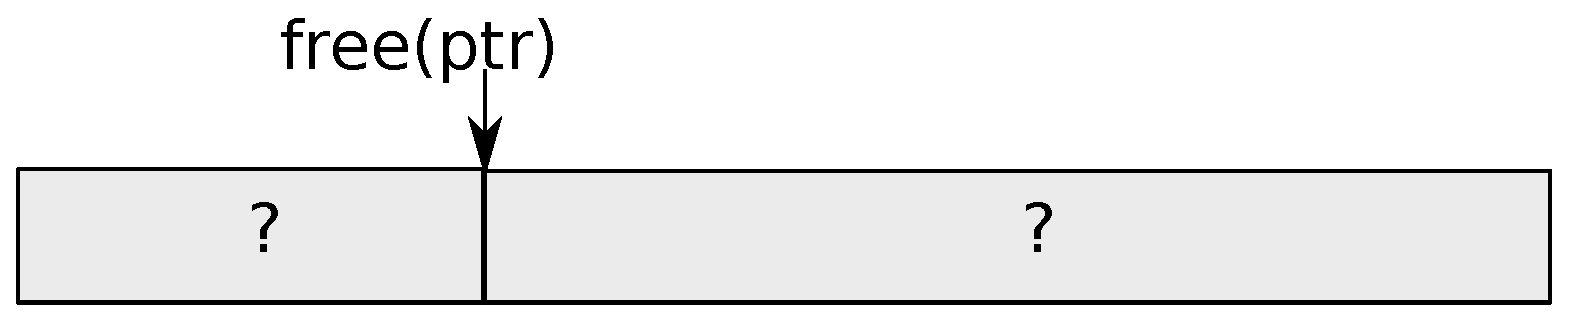
\includegraphics[width=.9\linewidth]{alloc-free0}

\onslide<2->{
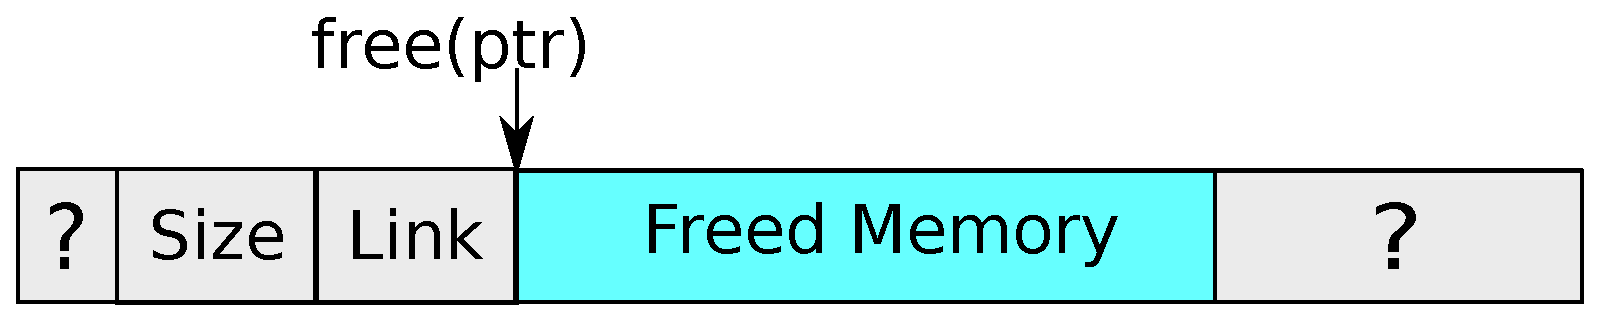
\includegraphics[width=.9\linewidth]{alloc-free1}
}

\end{frame}

\begin{frame}
\frametitle{Простые алгоритмы аллокации памяти}
\framesubtitle{Освобождение}

Самый простой вариант, просто добавить элемент в список (начало или конец):

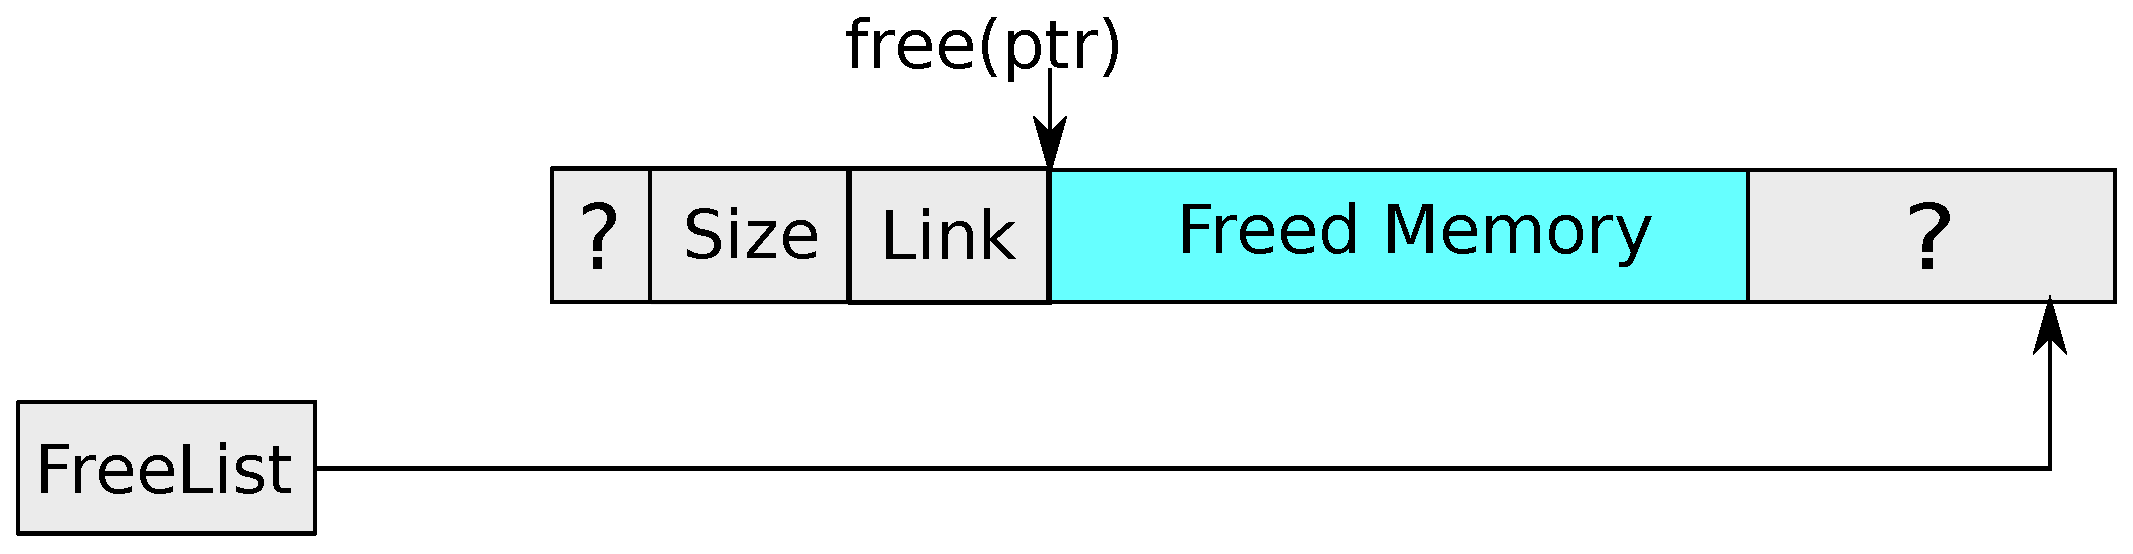
\includegraphics[width=.9\linewidth]{alloc-free2}

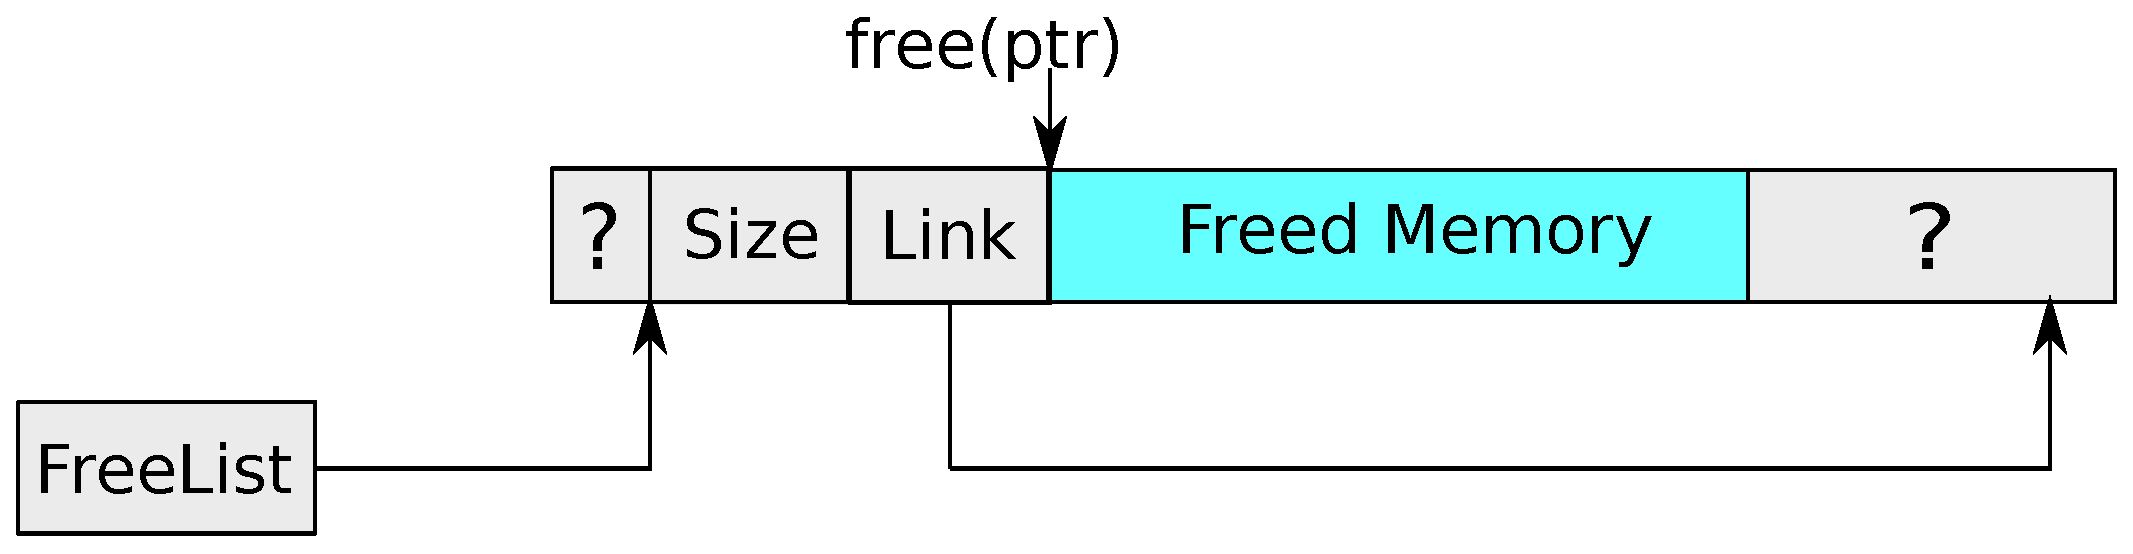
\includegraphics[width=.9\linewidth]{alloc-free3}

\end{frame}

\begin{frame}
\frametitle{Простые алгоритмы аллокации памяти}
\framesubtitle{Освобождение}

Рано или поздно это приведет к проблеме:

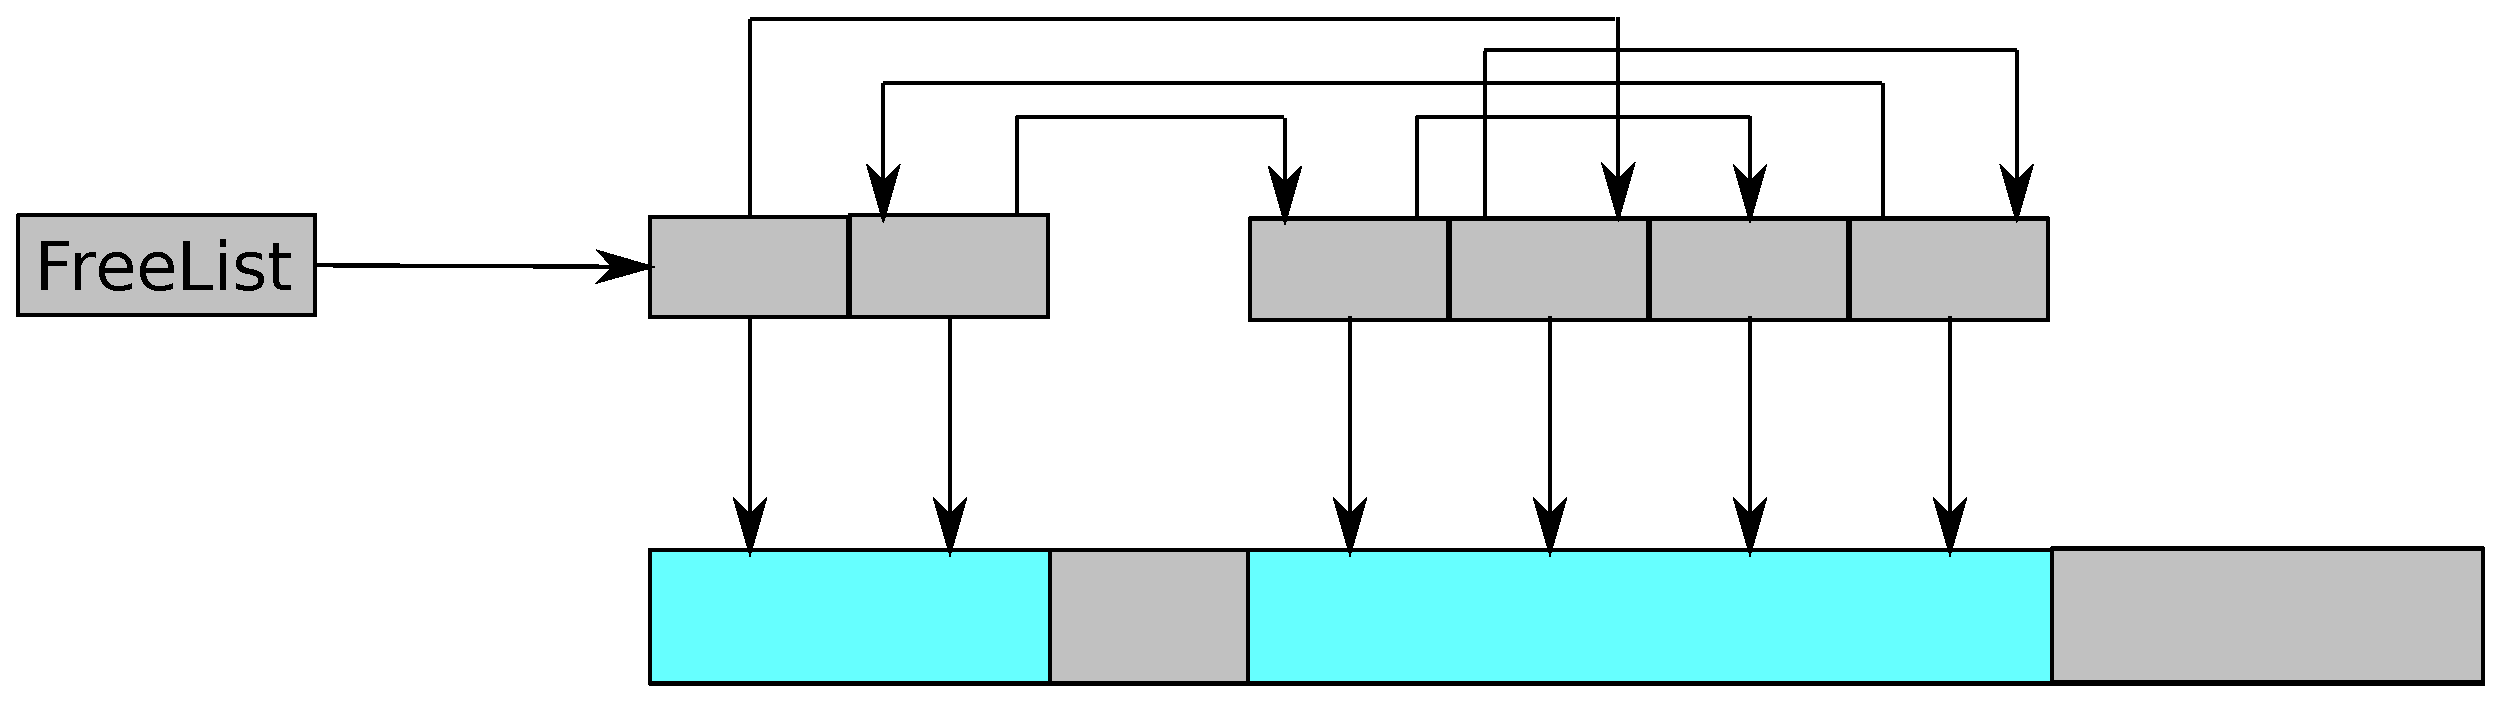
\includegraphics[width=.9\linewidth]{alloc-free4}

\end{frame}

\begin{frame}
\frametitle{Простые алгоритмы аллокации памяти}
\framesubtitle{Освобождение}

При освобождении необходимо объединять соседние свободные блоки:
\begin{itemize}
  \item<2-> чтобы не фрагментировать память, иначе мы не сможем аллоцировать большие участки памяти
  \item<3-> чтобы список свободных блоков не разрастался - плохо влияет на время аллокации памяти
\end{itemize}

\end{frame}

\begin{frame}
\frametitle{Простые алгоритмы аллокации памяти}
\framesubtitle{Освобождение}

Как объединять соседние свободные блоки:
\begin{itemize}
  \item<2-> мы можем поддерживать список отсортированным по адресу (классический версия malloc в UNIX, aka SLOB, описана в The C Programming Language)
  \item<3-> вместо списка можно использовать дерево - жертвуем памятью в обмен на производительность
  \item<4-> можно использовать Border Tags (авторство приписывают Кнуту, но идея очень очевидная)
\end{itemize}

\end{frame}

\begin{frame}
\frametitle{Простые алгоритмы аллокации памяти}
\framesubtitle{Освобождение}

Мы уже храним служебную информацию в начале блока, давайте добавим еще и в конец:
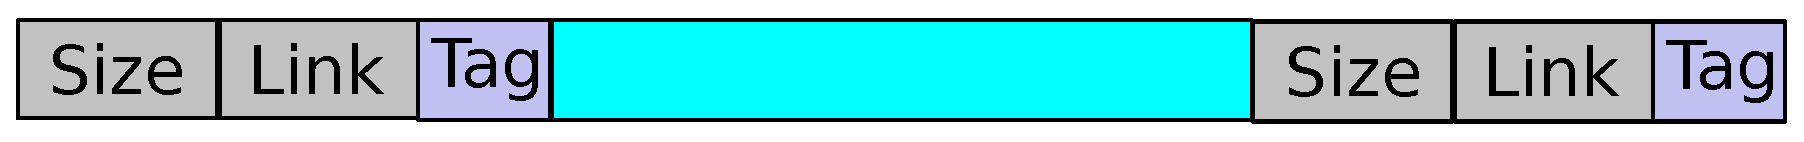
\includegraphics[width=.9\linewidth]{alloc-tag0}

\begin{itemize}
  \item<2-> TAG - индикатор свободности/занятости блока (это и есть Border Tag)
  \item<3-> Link-и в начале и в конце можно использовать как ссылки на следующий и ссылки на предыдущий блоки (просто для экономии памяти)
\end{itemize}

\end{frame}

\begin{frame}
\frametitle{Простые алгоритмы аллокации памяти}
\framesubtitle{Освобождение}

Мы знаем где находится Border Tag предыдущего (следующего) блока и можем легко
проверять свободность/занятость:
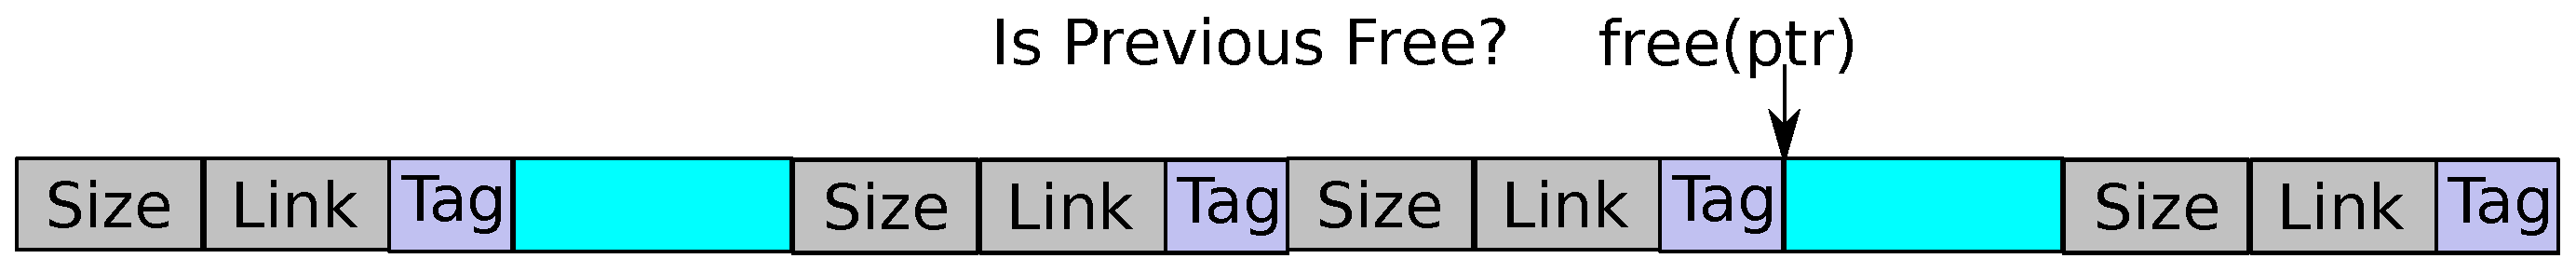
\includegraphics[width=.9\linewidth]{alloc-tag1}

\onslide<2->{
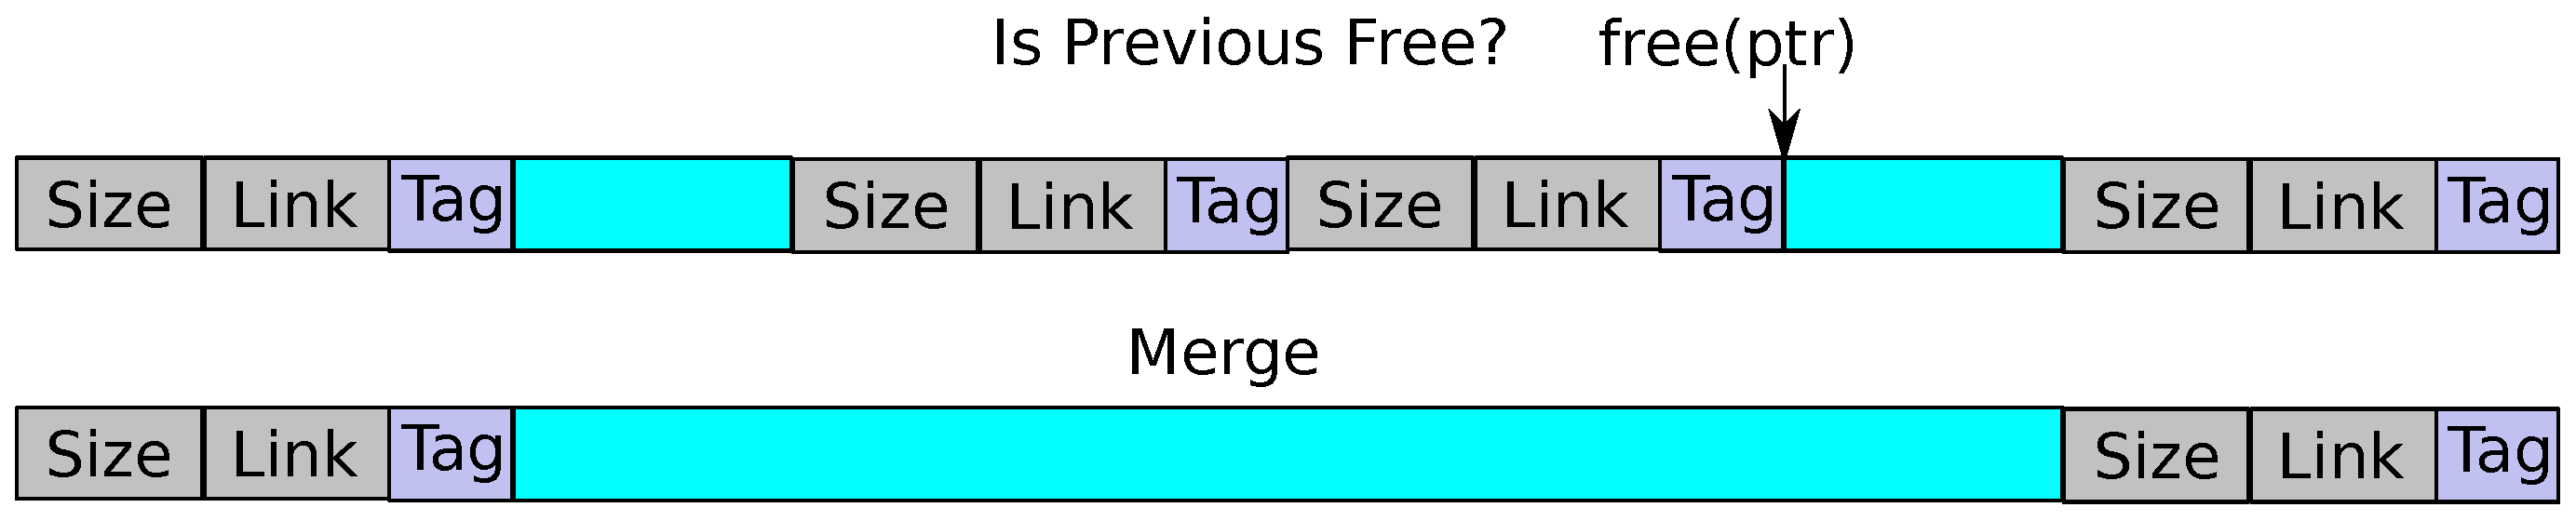
\includegraphics[width=.9\linewidth]{alloc-tag2}

При объединении сразу трех блоков нужно удалить один из двусвязного списка - O(1).
}

\end{frame}

  \begin{frame}
\frametitle{Продвинутые алгоритмы аллокации памяти}
\framesubtitle{Аллокация в несколько этапов}

Современные аллокаторы памяти выделяют две стадии:

\begin{itemize}
  \item<2-> аллокация больших блоков (Buddy Allocator и Ко.):
    \begin{itemize}
      \item аллокации происходят нечасто, большие объекты живут долго
      \item чем больше блок тем меньше накладные расходы на служебные структуры аллокатора - можем хранить больше информации
    \end{itemize}
  \item<3-> аллокация маленьких блоков фиксированного размера (SLAB и Ко.):
    \begin{itemize}
      \item блоки фиксированного размера проще аллоцировать
      \item блоки фиксированного размера требуют меньше служебной информации
      \item блоки имеют одинаковый размер не случайно - часто это объекты одного типа и это можно использовать
    \end{itemize}
\end{itemize}

\end{frame}

\begin{frame}
\frametitle{Buddy Allocator}
\framesubtitle{Вводные положения}

\begin{itemize}
  \item вся аллоцируемая память разбита на большие блоки фиксированного размера (будем называть их PAGE)
  \item каждому PAGE поставлен в соответствие дескриптор (мы легко можем получить дескриптор по номеру PAGE и наоборот, считайте, что у нас есть массив таких дескрипторов), хранящий служебную информацию (свободен/занят, порядок свободного блока)
  \item память аллоцируется и освобождается блоками по $2^i\times PAGE$, $i$ будем называть порядком блока
  \item порядок блока хранит пользователь и передает его в как функцию аллокации, так и в функцию освобождения
\end{itemize}
\end{frame}

\begin{frame}
\frametitle{Buddy Allocator}
\framesubtitle{Buddies}

Ключевой концепцией для Buddy Allocator-а является понятие Buddy:
\begin{itemize}
  \item Buddy Allocator хранит блоки в отдельных списках для каждого порядка (т. е. для каждого возможного порядка блока есть свой список), элементом списка является дескриптор первого PAGE в этом блоке;
  \item смежные (в памяти, а не в списке) блоки одного порядка называются Buddies (plural for buddy);
  \item два смежных блока (Buddies) в объединении дают один блок большего порядка, и наоборот из одного блока можно получить два Buddies меньшего порядка.
\end{itemize}

\end{frame}

\begin{frame}
\frametitle{Buddy Allocator}
\framesubtitle{Buddies}

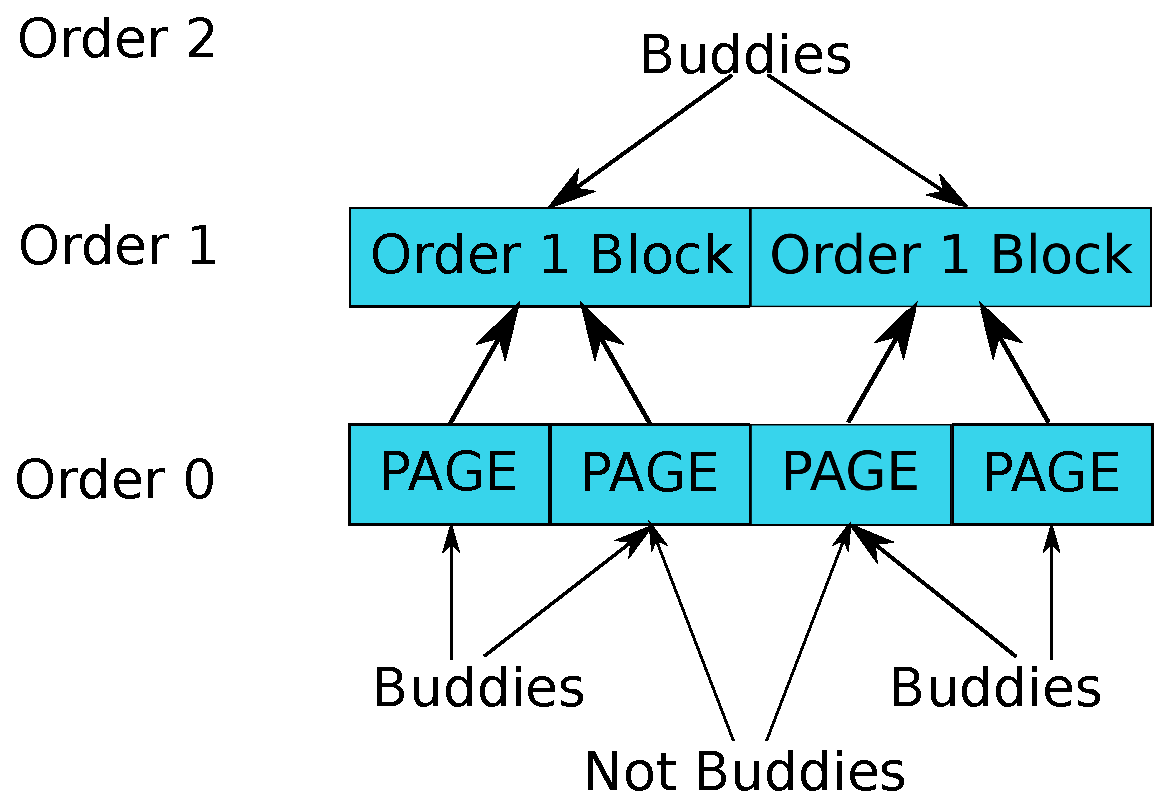
\includegraphics[width=.9\linewidth]{buddy-buddies}

\end{frame}

\begin{frame}
\frametitle{Buddy Allocator}
\framesubtitle{Аллокация}

Аллокация блока порядка $i$ происходит из списка соответствующего блокам порядка $i$:

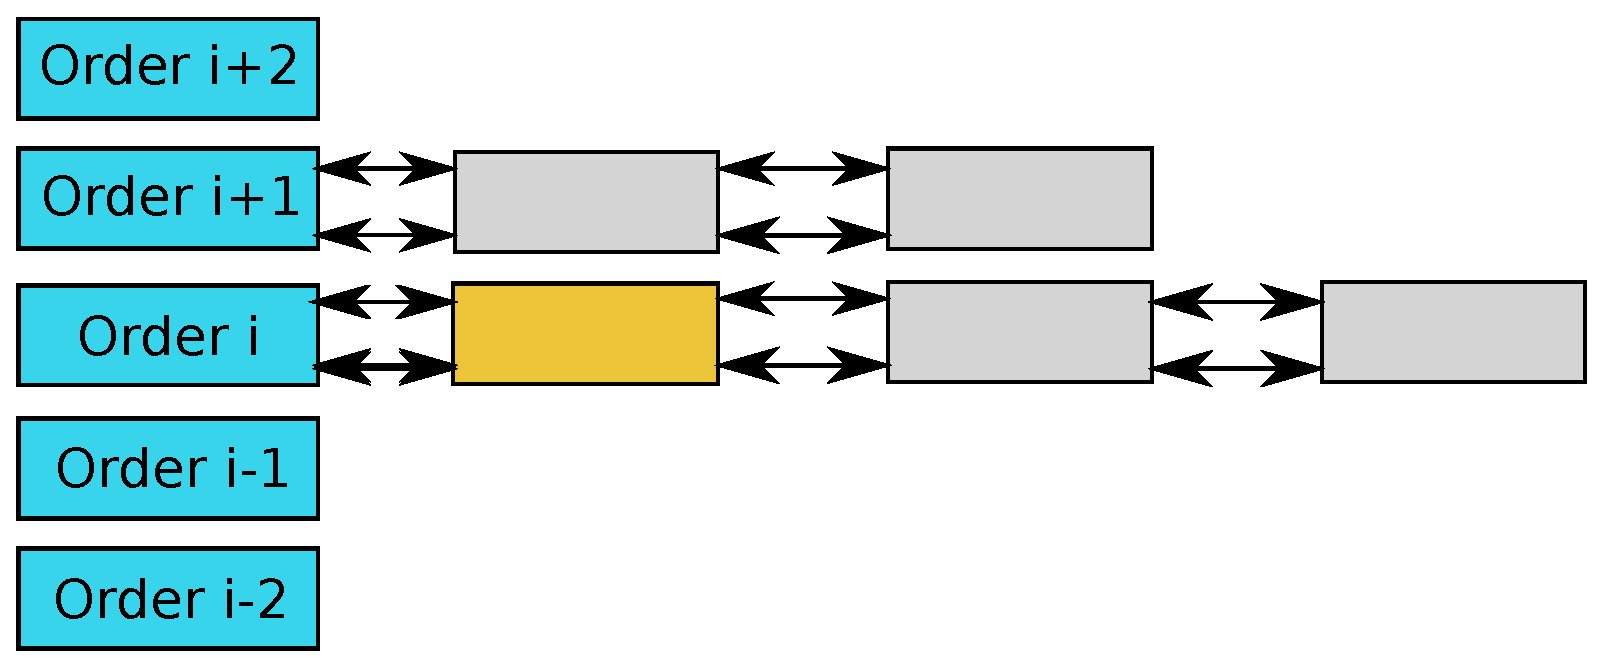
\includegraphics[width=.9\linewidth]{buddy-alloc0}

\end{frame}

\begin{frame}
\frametitle{Buddy Allocator}
\framesubtitle{Аллокация}

Если список пуст, ищем не пустой список большего порядка и аллоцируем из него, например, аллоцируем блок порядка $i-2$:

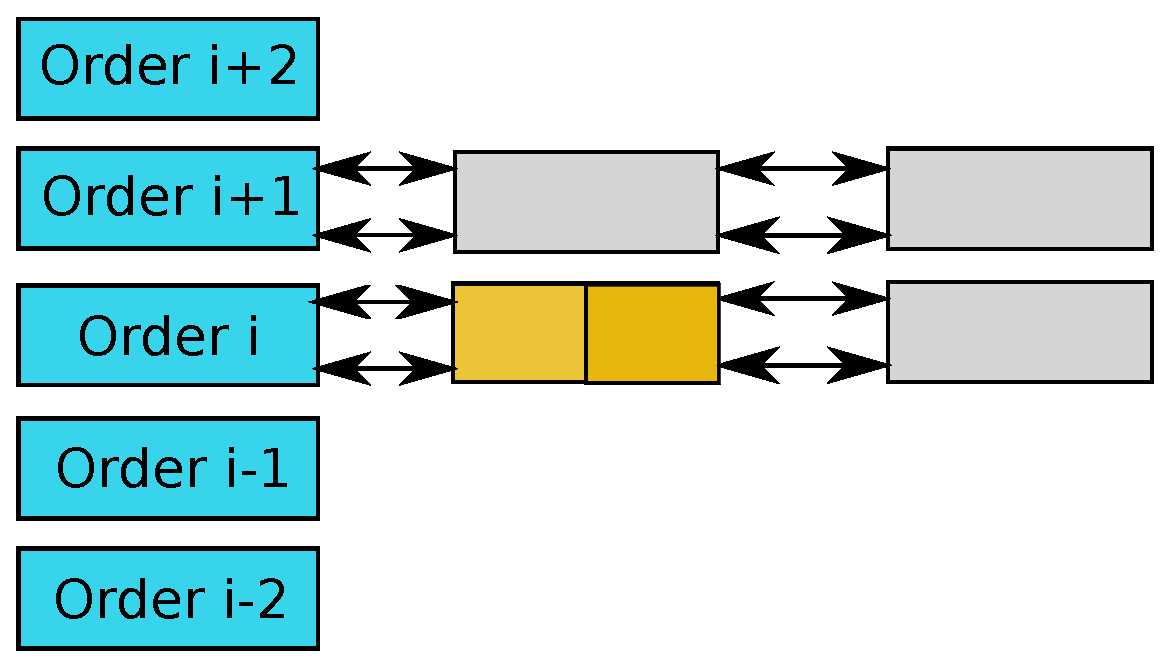
\includegraphics[width=.8\linewidth]{buddy-alloc1}

\end{frame}

\begin{frame}
\frametitle{Buddy Allocator}
\framesubtitle{Аллокация}

Блок порядка $i$ слишком большой, поэтому делим его на две части порядка $i-1$ и одну из частей возвращаем аллокатору:

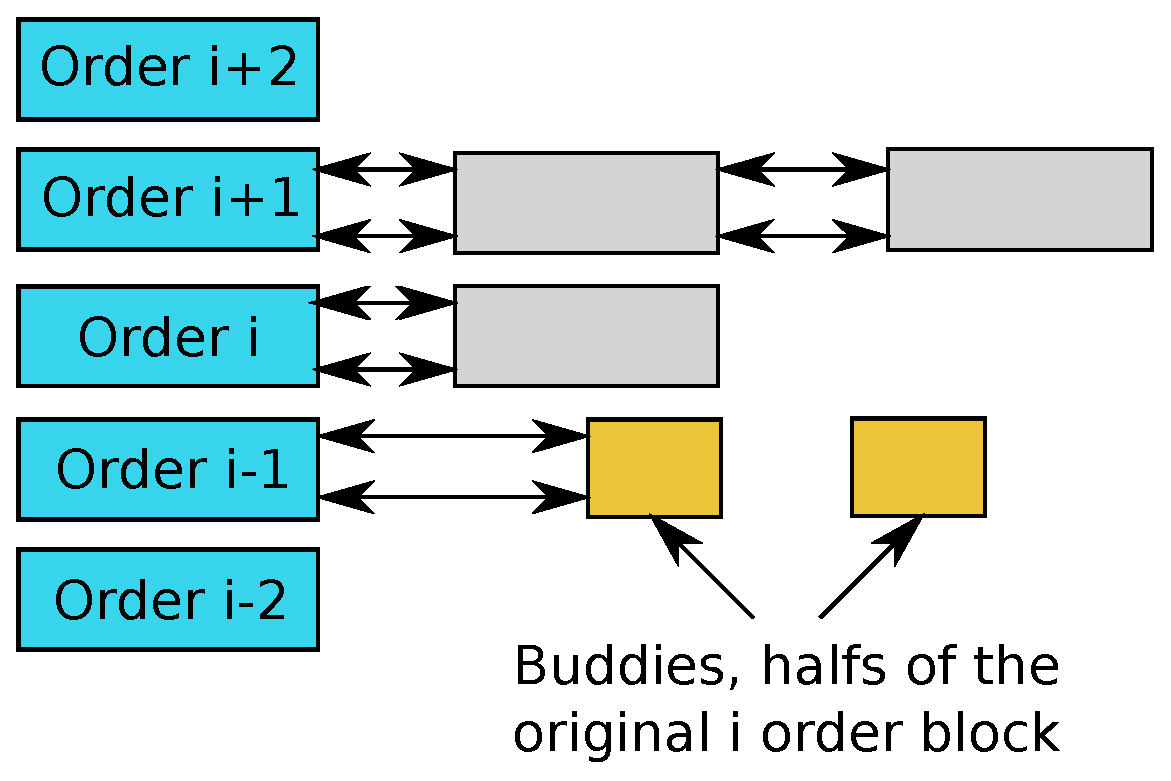
\includegraphics[width=.8\linewidth]{buddy-alloc2}

\end{frame}

\begin{frame}
\frametitle{Buddy Allocator}
\framesubtitle{Аллокация}

Продолжаем пока не дойдем до нужного порядка:

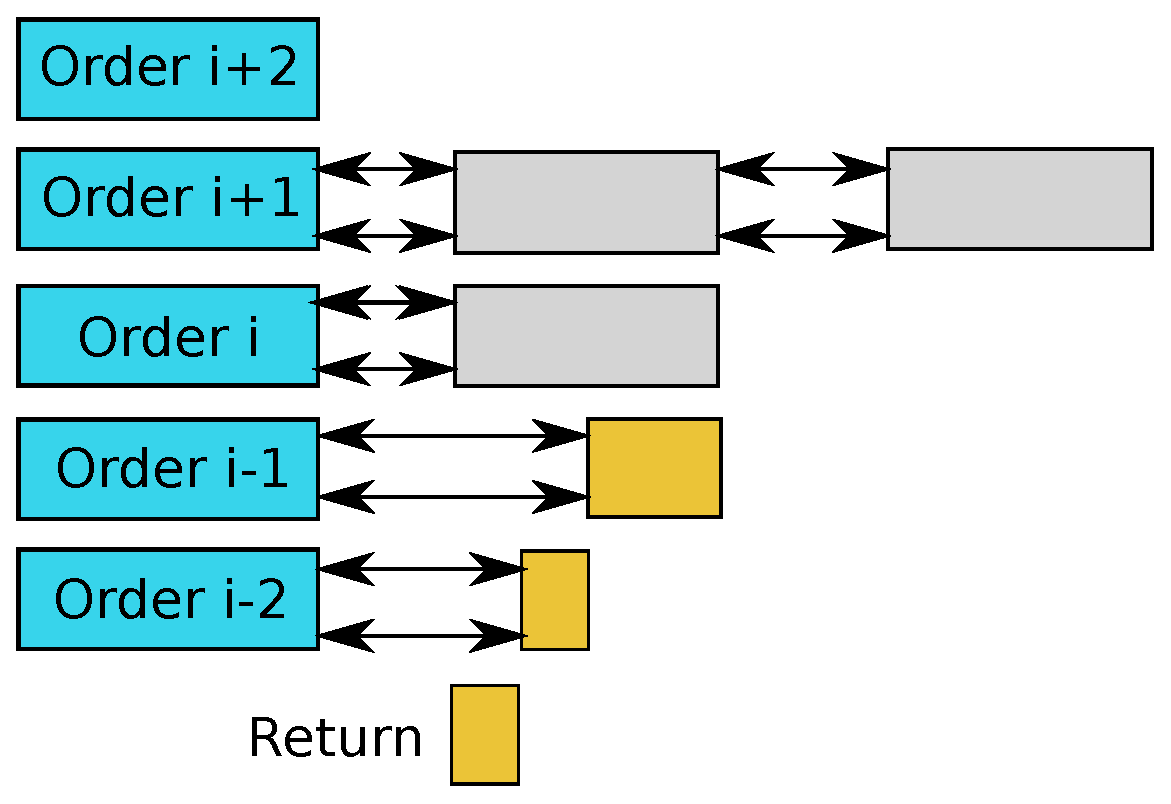
\includegraphics[width=.8\linewidth]{buddy-alloc3}

\end{frame}

\begin{frame}
\frametitle{Buddy Allocator}
\framesubtitle{Аллокация}

Каждый свободный блок, как отмечалось выше представляется дескриптором первого PAGE, дескриптор должен хранить:

\begin{itemize}
  \item признак занятости и свободности блока;
  \item порядок блока, "головой" которого является данный PAGE.
\end{itemize}

Эта информация не нужна для аллокации, но понадобится для освобождения, поэтому
при разделении блока необходимо обновить дескрипторы обоих половин.

\end{frame}

\begin{frame}
\frametitle{Buddy Allocator}
\framesubtitle{Освобождение}

При освобождении необходимо объединять смежные блоки (Buddies), чтобы избежать фрагментации. Найти "голову" смежного блока легко:

\[
	Buddy_{No} = Head_{No} \char`\^ (1 << i)
\]

где
\begin{itemize}
  \item $Buddy_{No}$ - номер PAGE, являющегося "головой" смежного блока;
  \item $Head_{No}$ - номер PAGE, являющегося "головой" блока, с которым мы работаем;
  \item $i$ - порядок блока;
\end{itemize}

\end{frame}

\begin{frame}
\frametitle{Buddy Allocator}
\framesubtitle{Освобождение}

Освобождаемый блок можно объединить со смежным (Buddy), только если смежный блок свободен. Смежный блок свободен если:

\begin{itemize}
  \item в дескрипторе "головы" блока установлен признак свободности;
  \item порядок сохраненный в дескрипторе "головы" блока совпадает с порядком освобождаемого блока.
\end{itemize}
\end{frame}

\begin{frame}
\frametitle{Buddy Allocator}
\framesubtitle{Освбождение}

Прядок блоков важен при объединении:
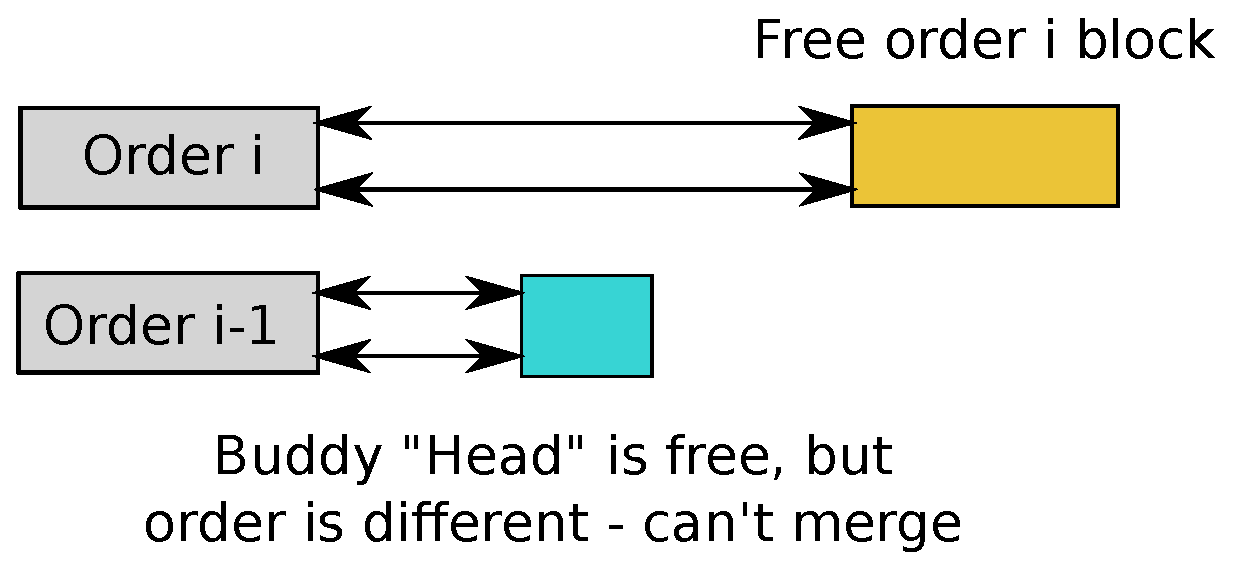
\includegraphics[width=.9\linewidth]{buddy-free0}
\end{frame}

\begin{frame}
\frametitle{Buddy Allocator}
\framesubtitle{Освобождение}

Возможно придется сделать несколько объединений:
\only<1>{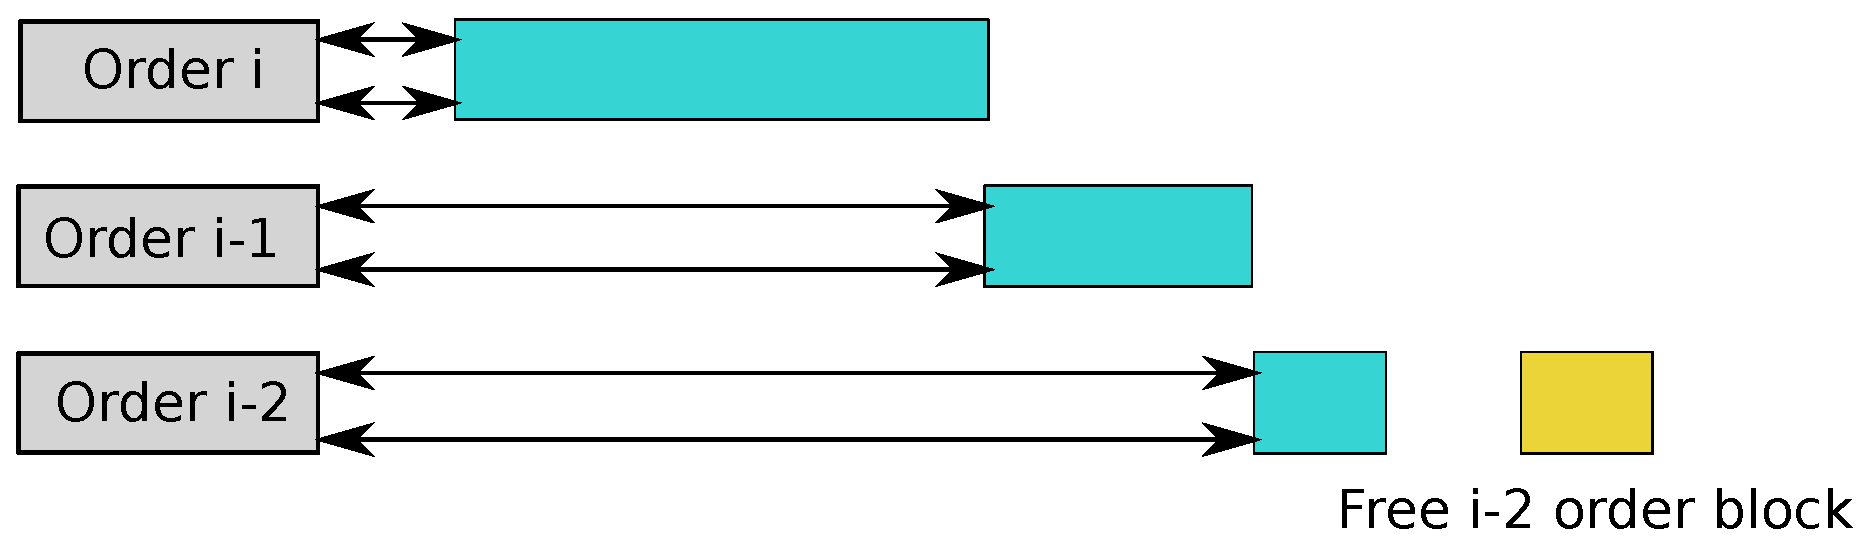
\includegraphics[width=.9\linewidth]{buddy-free1}}
\only<2>{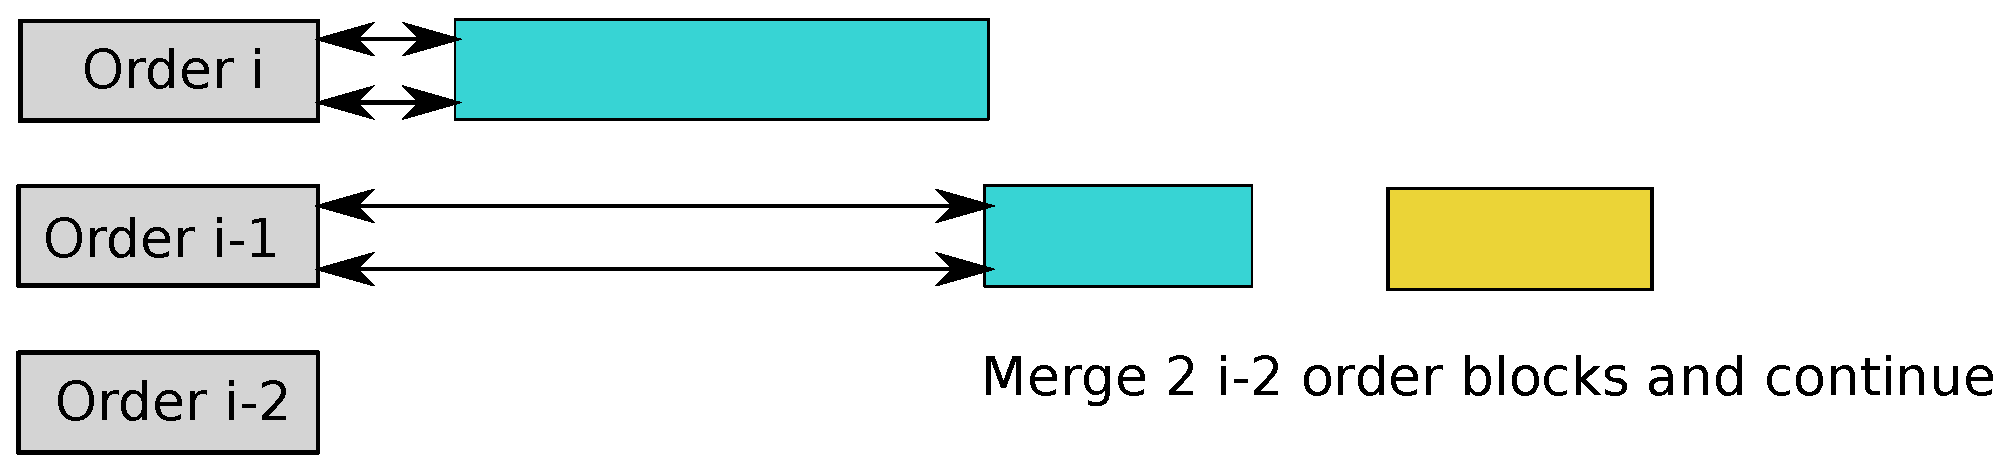
\includegraphics[width=.9\linewidth]{buddy-free2}}
\only<3>{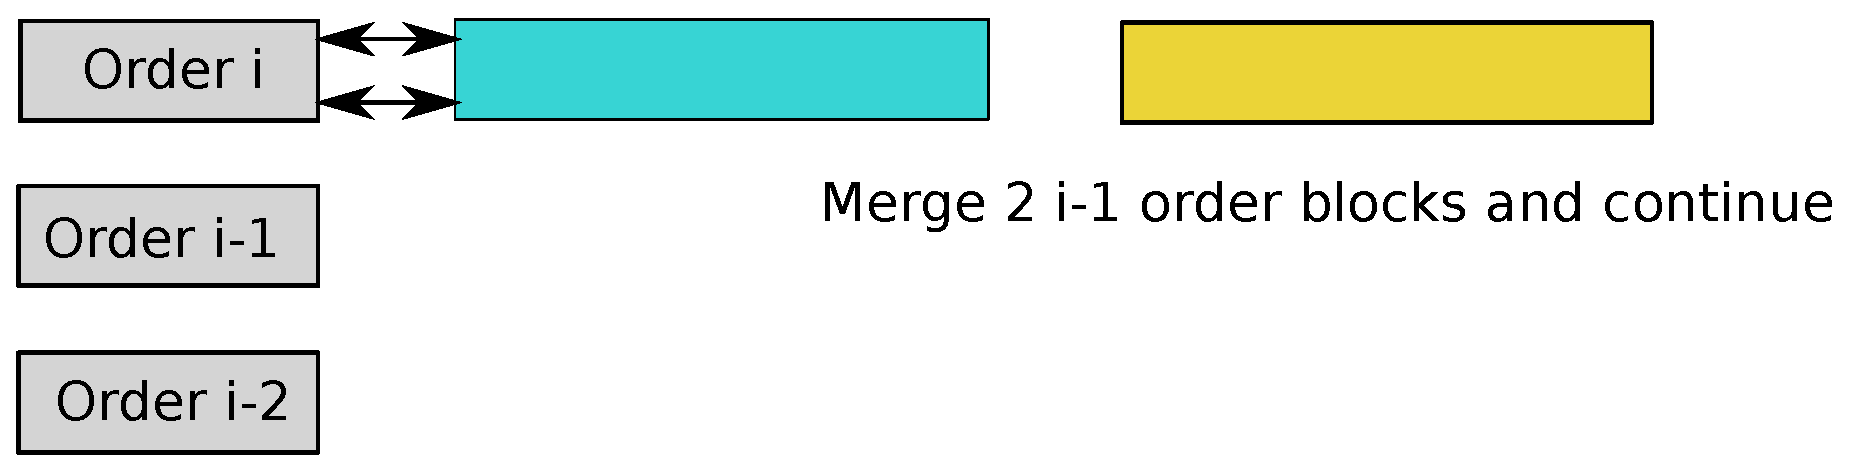
\includegraphics[width=.9\linewidth]{buddy-free3}}

\end{frame}

\begin{frame}
\frametitle{Buddy Allocator}
\framesubtitle{Освобождение}

Продолжаем пока можем объединять смежные блоки или не дойдем до последнего уровня:
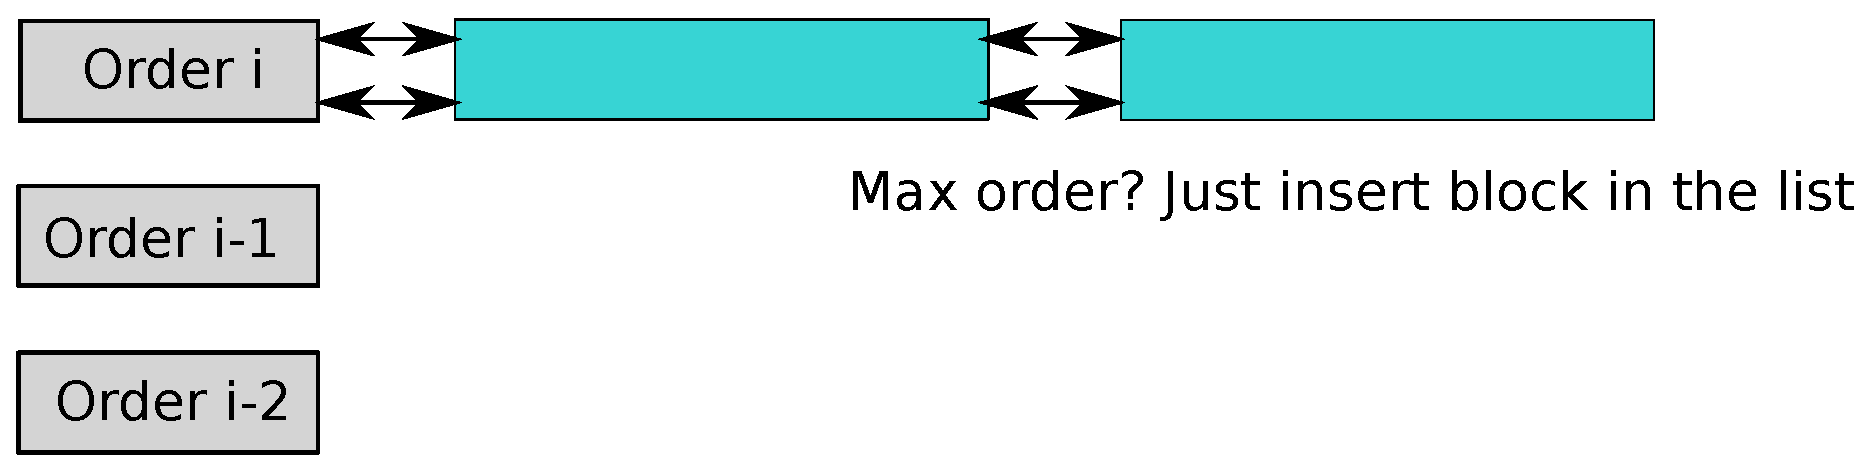
\includegraphics[width=.9\linewidth]{buddy-free4}
\end{frame}

\begin{frame}
\frametitle{Buddy Allocator}
\framesubtitle{Аллокация блоков произвольного размера}

Аллокация блоков только по степеням 2 может быть затратной - в неудачных случаях мы аллоцируем почти в 2 раза больше чем нужно. Есть как минимум 2 решения этой проблемы:

\begin{itemize}
  \item пожертвовать интерфейсом - разложить количество блоков на сумму степеней 2 и аллоцировать каждый блок размера $2^i$ отдельно и возвращать массив блоков;
  \item поправить алгоритм для аллокация блоков произвольного размера;
\end{itemize}
\end{frame}

\begin{frame}
\frametitle{Buddy Allocator}
\framesubtitle{Аллокация блоков произвольного размера}

Buddy Allocator легко изменить для аллокации блоков произвольного размера пожертвовав (совсем немного) памятью:
\begin{itemize}
  \item вместо порядка блока в дескрипторе PAGE храним размер (очевидно);
  \item храним признак занятости/свободности и размер как в дескрипторе первого PAGE блока, так и в дескрипторе последнего (Border Tags);
  \item каждый список хранит блоки размеров $\left[2^i;2^{i+1}\right)$, кроме последнего - для него нет верхней границы.
\end{itemize}
\end{frame}

  \begin{frame}
\frametitle{SLAB Allocator}
\framesubtitle{Аллокация маленьких объектов фиксированного размера}

Теперь решаем еще более простую задачу - аллокацию "маленьких" объектов фиксированного размера:
\begin{itemize}
  \item мы умеем аллоцировать большие блоки - будем использовать их как пулы;
  \item аллоцируем блоки фиксированного размера из пула - тривиально;
  \item объекты одного размера уменьшают вероятность фрагментации;
  \item как на этом построить универсальный аллокатор (malloc/free)?
\end{itemize}

\end{frame}

\begin{frame}
\frametitle{SLAB Allocator}

Базовым понятием для SLAB аллокатора является (неожиданно) SLAB:
\begin{itemize}
  \item SLAB - это пулл объектов одинакового размера;
  \item аллокатор может иметь в распоряжении несколько SLAB-ов - при необходимости аллоцируются новые SLAB-ы;
  \item каждому объекту в SLAB-е соответствует дескриптор (по сути, нужен, чтобы связать объекты в список);
\end{itemize}
\end{frame}

\begin{frame}
\frametitle{SLAB Allocator}
\framesubtitle{Разделение на большие и маленькие объекты}

SLAB аллокатор делит объекты далее на большие и маленькие, и использует для них разную структуру SLAB-ов:
\begin{itemize}
  \item разделение нужно чтобы уменьшить потери памяти для больших объектов;
  \item нет четкой границы, что считать большим объектом, а что маленьким;
  \item обычно маленькими объектами считают объекты меньше $1/8$ размера PAGE (минимального размера пула).
\end{itemize}

\end{frame}

\begin{frame}
\frametitle{SLAB Allocator}
\framesubtitle{Организация SLAB-а маленьких объектов}

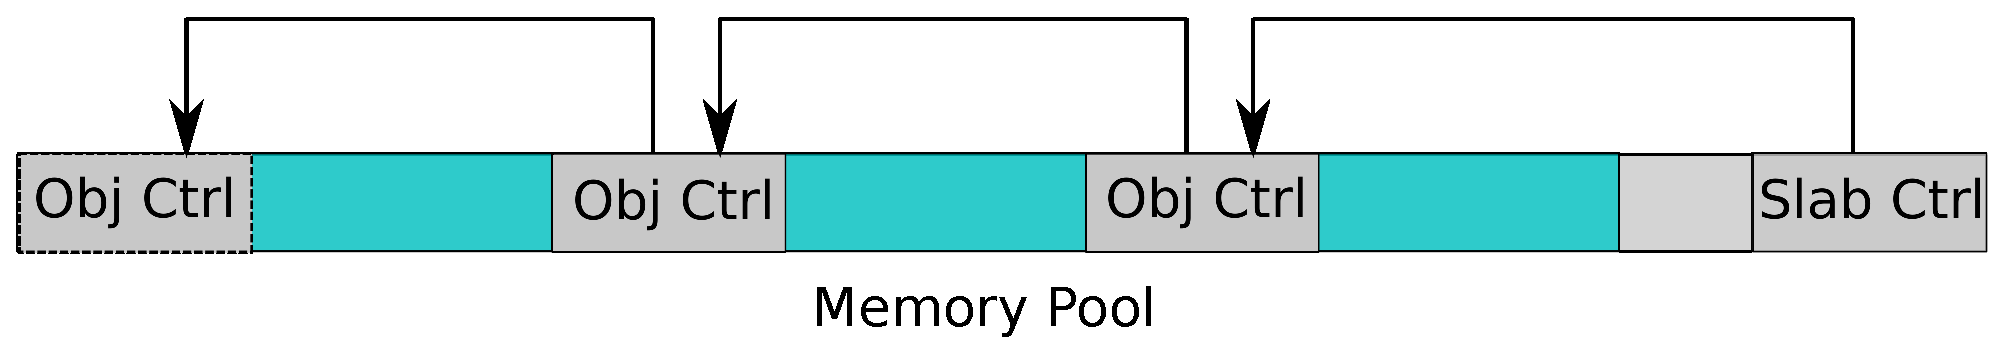
\includegraphics[width=.9\linewidth]{slab-small}

\end{frame}

\begin{frame}
\frametitle{SLAB Allocator}
\framesubtitle{Организация SLAB-а больших объектов объектов}

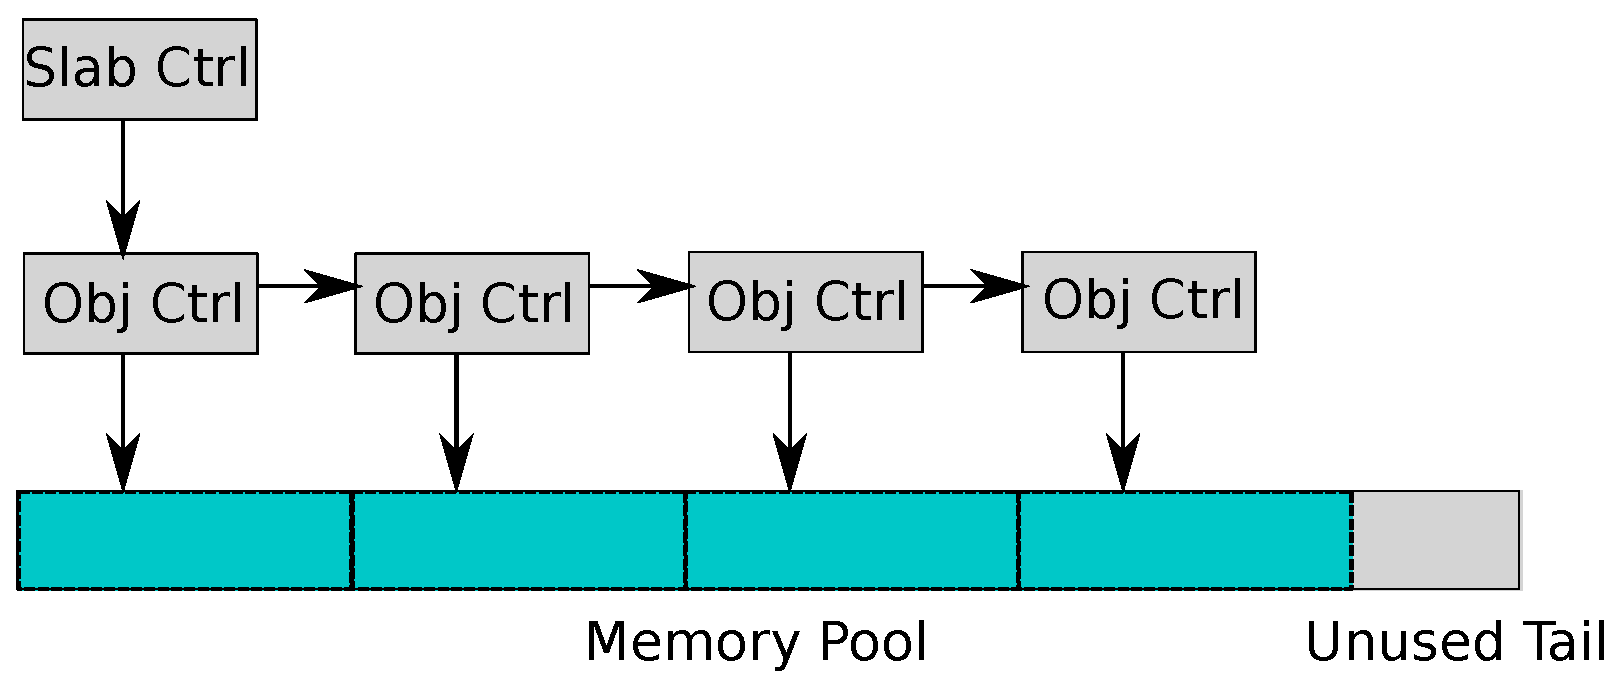
\includegraphics[width=.9\linewidth]{slab-large}

\end{frame}

\begin{frame}
\frametitle{SLAB Allocator}
\framesubtitle{Детали реализации}

\begin{itemize}
  \item Для SLAB-ов больших объектов управляющие структуры нужно аллоцировать отдельно - используя SLAB-ы маленьких объектов.
  \item При освобождении объекта нам нужно найти SLAB из которого он аллоцирован, это можно делать используя словарь (dict, map) или (гораздо проще) используя дескриптор PAGE.
  \item Для SLAB-ов больших объектов ObjCtrl необходим только когда объект свободен, когда объект объект был аллоцирован ObjCtrl больше не нужен.
\end{itemize}
\end{frame}

\begin{frame}
\frametitle{SLAB Allocator}
\framesubtitle{malloc/free}

Используя Buddy Allocator и Slab Allocator можно создать аллокатор общего назначения (malloc/free):
\begin{itemize}
  \item Buddy Allocator - для аллокации пулов памяти для SLAB-ов и для аллокации памяти для больших объектов;
  \item набор предварительно созданных SLAB Allocator-ов с разными размерами объектов - для аллокации маленьких объектов;
\end{itemize}
\end{frame}

\begin{frame}
\frametitle{SLAB Allocator}
\framesubtitle{Объекты одного типа}

Мы можем создавать SLAB Allocator-ы под специфичные нужды и не использовать аллокатор общего назначения:
\begin{itemize}
  \item можно повысить надежность - уменьшив вероятность, что кто-то, по ошибке, испортит нашу память, или, наоборот, что мы испортим чужую;
  \item меньше конкуренция за ресурсы - аллокатором общего назначения пользуются все, а специальным аллокатором только мы;
  \item можно сэкономить на инициализации (далее подробнее);
\end{itemize}
\end{frame}

\begin{frame}
\frametitle{SLAB Allocator}
\framesubtitle{Объекты одного типа}

Многие поля объекта естественным образом оказываются в "инициализированном" состоянии при освобождении объекта:

\begin{itemize}
  \item если объект хранит mutex или spinlock (или какой-то другой примитив синхронизации), то перед освобождением он должен быть отпущен;
  \item если объект хранит счетчик ссылок, то перед освобождением он, зачастую, равен нулю;
  \item если объект хранит список или корень дерева, то перед освобождением они, зачастую, будут пустыми;
\end{itemize}

Такие поля достаточно инициализировать один раз -- экономия на инициализации.

\end{frame}

\begin{frame}
\frametitle{SLAB Allocator}
\framesubtitle{Cache Coloring}

Иногда, при использовании SLAB Allocator-а для достаточно больших объектов, в пуле памяти могут быть неиспользуемые "хвосты" - размер пула не делится нацело на размер объекта.

Этим неиспользуемым хвостам можно найти полезное применение - Cache Coloring.

\end{frame}

\begin{frame}
\frametitle{SLAB Allocator}
\framesubtitle{Cache Coloring}

\begin{columns}[T]

  \begin{column}{.3\textwidth}
    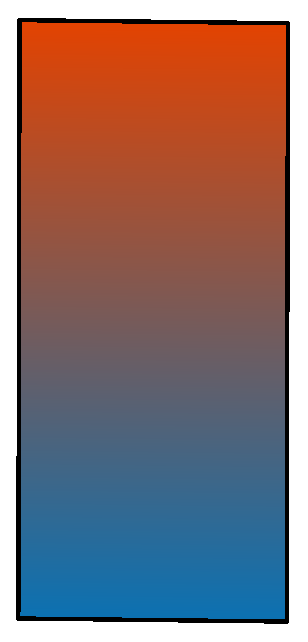
\includegraphics[width=.8\linewidth]{obj-hotmap}
  \end{column}

  \begin{column}{.7\textwidth}
    \begin{itemize}
      \item "горячие" поля, обычно, в начале:
        \begin{itemize}
          \item указатели (следующий/предыдущий, левый/правый)
          \item ключи для поиска (обычно короткие)
          \item флаги и примитивы синхронизации
        \end{itemize}
      \item "холодные" поля, обычно, в конце:
        \begin{itemize}
          \item значения, которые мы ищем (могут быть большими)
        \end{itemize}
    \end{itemize}
  \end{column}

\end{columns}

\end{frame}

\begin{frame}
\frametitle{SLAB Allocator}
\framesubtitle{Cache Coloring}

\begin{columns}[T]

  \begin{column}{.3\textwidth}
    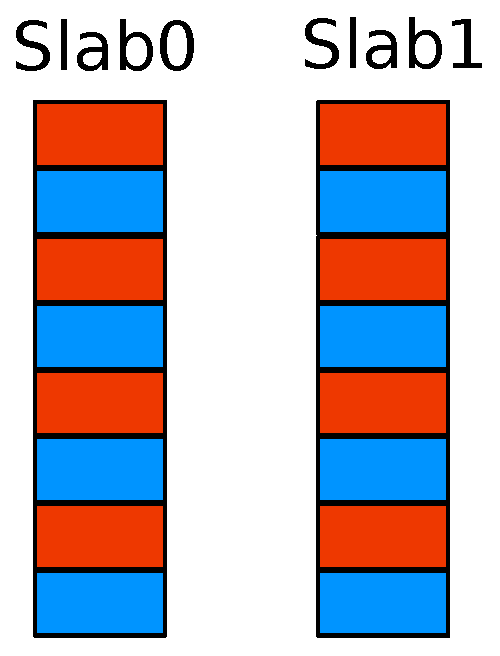
\includegraphics[width=\linewidth]{slab-color0}
  \end{column}

  \begin{column}{.7\textwidth}
    \begin{itemize}
      \item "горячие" поля объектов в Slab0 конкурируют с "горячими" полями объектов в Slab1 за место в процессорном кеше
      \item "холодные" поля конкурируют с "холодными" полями
      \item "холодные" поля используются редко - растрата кеша, лучше поделить его между "горячими" полями
    \end{itemize}
  \end{column}

\end{columns}

\end{frame}

\begin{frame}
\frametitle{SLAB Allocator}
\framesubtitle{Cache Coloring}

\begin{columns}[T]

  \begin{column}{.3\textwidth}
    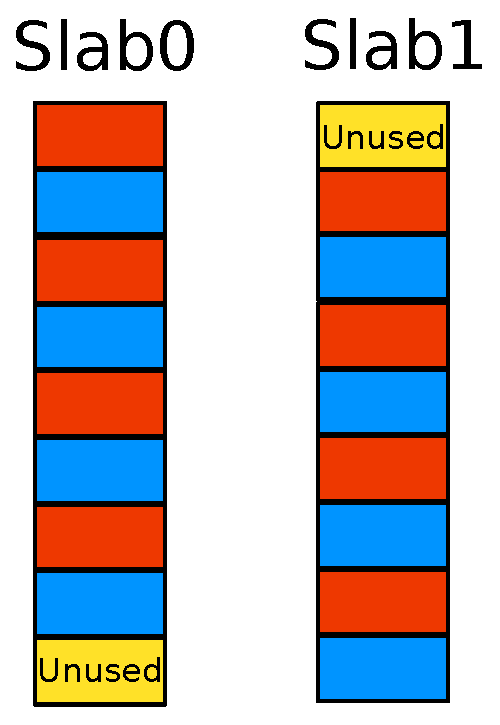
\includegraphics[width=\linewidth]{slab-color1}
  \end{column}

  \begin{column}{.7\textwidth}
    \begin{itemize}
      \item "горячие" поля объектов в Slab0 и Slab1 занимают весь кеш
      \item "холодные" поля поднимаются в кеш, только когда они нужны
    \end{itemize}
  \end{column}

\end{columns}

\end{frame}


  \begin{frame}
\frametitle{Ссылки}

\begin{itemize}
  \item The Art of Computer Programming. Volume 1, 2.5. Donald Knuth - обзор простых алгоритмов аллокации и их поведения;
  \item The Slab Allocator: An Object-Caching Kernel Memory Allocator. Jeff Bonwick - описание классического SLAB Allocator-а;
  \item Magazines and Vmem: Extending the Slab Allocator to Many CPUs and Arbitraray Resources. Jeff Bonwick, Jonathan Adams - продолжение истории SLAB Allocator-а;
  \item Slab allocators in the Linux Kernel: SLAB, SLOB, SLUB. Christoph Lameter - о реализации кеширующих аллокаторов в ядре Linux.
\end{itemize}
\end{frame}


%  \begin{frame}
%    \bibliography{lec1}{}
%    \bibliographystyle{apalike}
%  \end{frame}

\end{document}
